\section{目的}
  1週目では紙の上で回路設計を行ったが,巨大なシステム,例えばGPU\footnote{Graphics Processing Unitの略} などを
    紙上で設計することは困難であり,コンピュータを用いて設計することが一般的である.
  2週目では,近年の回路設計技術に対する理解を深めるために,Windowsツール,Xilinx ISE WebPACKを用いて回路設計を行う.
  また,回路シミュレータ上で動作検証を行う.

  \subsection{Xilinx ISE WebPACKについて}
  一般に集積回路の制作には時間がかかり,また大量生産を行わない限りコストもかかるため,
  少量生産を行う際はFPGA\footnote{Field Programmable Gate Arrayの略} など論理回路をエミュレートできる回路が使用される.
  Xilinx は FPGA の大手メーカであり,ISE WebPACK は Xilinx が提供する.

\section{実験方法}
シミュレーションで使用するデバイスは Spartan3E ファミリの XC3S100E の CP132 パッケージである.
Xilinxの回路図ベースで実験を進めていく.
\subsection{課題1 3入力多数決回路}
3入力多数決回路の回路を作成する.真理値表を表\ref{tab:TMR}に示す.
\begin{table}[htb]
  \centering
  \caption{多数決回路の真理値表}
  \label{tab:TMR}
  \begin{tabular}{ccc|c}
    $A$ & $B$ & $C$ & $Y$ \\ \hline
     0  &  0  &  0  &  0  \\
     0  &  0  &  1  &  0  \\
     0  &  1  &  0  &  0  \\
     0  &  1  &  1  &  1  \\
     1  &  0  &  0  &  0  \\
     1  &  0  &  1  &  1  \\
     1  &  1  &  0  &  1  \\
     1  &  1  &  1  &  1  \\
  \end{tabular}
\end{table}
設計した回路図を\ref{fig:TMRsch}に示す.
シミュレーションのテストベンチを付録のソースコード\ref{lst:tmrtestbench}に示す.

\begin{figure}[tbp]
   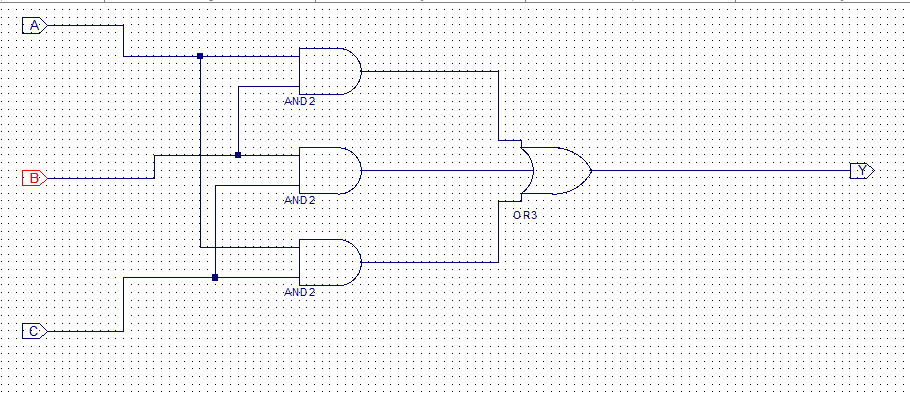
\includegraphics[width=150mm,angle=0]{week2/pics/TMRsch.png}
   \caption{3入力多数決回路の回路図} %タイトルをつける
   \label{fig:TMRsch} %ラベルをつけ図の参照を可能にする
\end{figure}

\subsection{課題2 発展課題 10進7セグデコーダの制作}
7セグメントデコーダを作成する.$I_0$から$I_3$の入力で7セグメント LED のセグメントの出力を得るようにする.
設計する回路は,正論理を仮定すると,アノードコモンの7セグメント LED は0のときに光るようにする.
そのため真理値表は表\ref{tab:7segdec}のとおりである.
カルノー図を半自動生成するために Excel を用いて表を生成している(図\ref{fig:7seg-dec-des}).
シミュレーションのテストベンチを付録のソースコード\ref{lst:schbased7segtestbench}に示す.

\begin{table}[htb]
  \centering
  \caption{7セグデコーダの真理値表}
  \label{tab:7segdec}
  \begin{tabular}{c||cccc||ccccccc}
     N &$I_3$&$I_2$&$I_1$&$I_0$&$A$&$B$&$C$&$D$&$E$&$F$&$G$ \\ \hline
     0 & 0  &  0  &  0  &  0 & 0 & 0 & 0 & 0 & 0 & 0 & 1 \\
     1 & 0  &  0  &  0  &  1 & 1 & 0 & 0 & 1 & 1 & 1 & 1 \\
     2 & 0  &  0  &  1  &  0 & 0 & 0 & 1 & 0 & 0 & 1 & 0 \\
     3 & 0  &  0  &  1  &  1 & 0 & 0 & 0 & 0 & 0 & 0 & 1 \\
     4 & 0  &  1  &  0  &  0 & 1 & 0 & 0 & 1 & 1 & 0 & 0 \\
     5 & 0  &  1  &  0  &  1 & 0 & 1 & 0 & 0 & 1 & 0 & 0 \\
     6 & 0  &  1  &  1  &  0 & 0 & 1 & 0 & 0 & 0 & 0 & 0 \\
     7 & 0  &  1  &  1  &  1 & 0 & 0 & 0 & 1 & 1 & 1 & 1 \\
     8 & 1  &  0  &  0  &  0 & 0 & 0 & 0 & 0 & 0 & 0 & 0 \\
     9 & 1  &  0  &  0  &  1 & 0 & 0 & 0 & 0 & 1 & 0 & 0 \\
  \end{tabular}
\end{table}

\begin{figure}[tbp]
   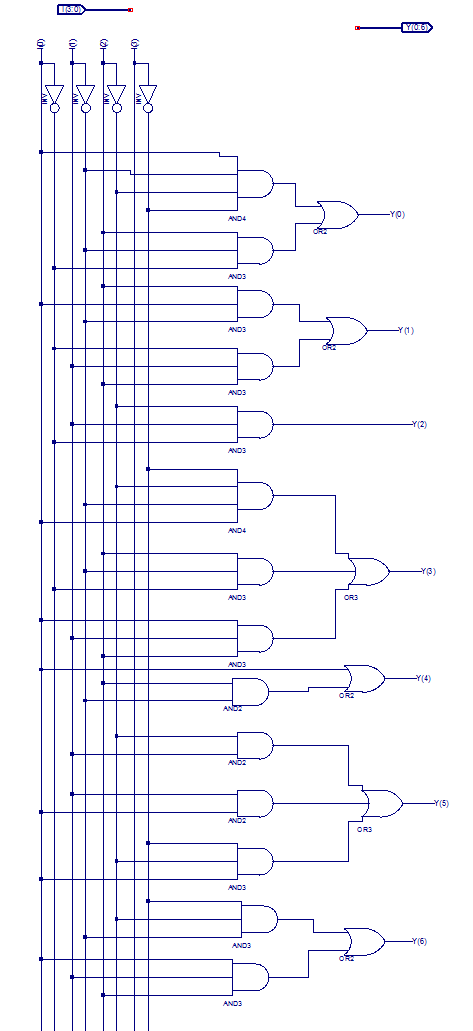
\includegraphics[height=230mm,angle=0]{week2/pics/7seg-sch.png}
   \caption{7セグデコーダの回路図} %タイトルをつける
   \label{fig:7seg-dec-sch} %ラベルをつけ図の参照を可能にする
\end{figure}

\begin{figure}[tbp]
   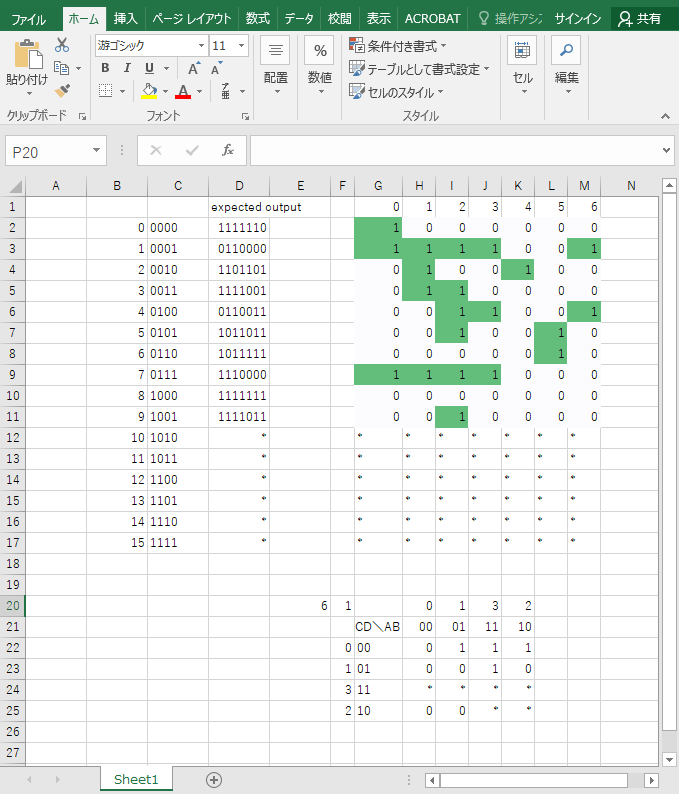
\includegraphics[width=150mm,angle=0]{week2/pics/designingprocess.png}
   \caption{7セグデコーダの設計に用いたシート, 画像では6のカルノー図が出力されている} %タイトルをつける
   \label{fig:7seg-dec-des} %ラベルをつけ図の参照を可能にする
\end{figure}


\subsection{課題3 2入力ANDゲートのFPGAボードでの動作確認}
2入力ANDゲートを実際に作成し,その入力を押しボタンスイッチ,出力をLEDに接続し,入出力を割り当て,
コンフィグレーションデータを作成する.
作成したデータをFPGAにダウンロードし,動作検証をする.
回路図を図\ref{fig:ANDsch}に示す.ピンのa割り当てを図\ref{fig:ANDpinasign}に示す.

\begin{figure}[tbp]
  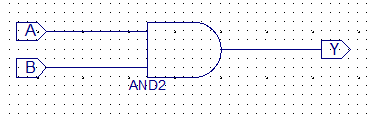
\includegraphics[width=100mm,angle=0]{week2/pics/ledswandsch.png}
  \centering
   \caption{ANDゲートの回路図} %タイトルをつける
   \label{fig:ANDsch} %ラベルをつけ図の参照を可能にする
\end{figure}


\begin{figure}[tbp]
  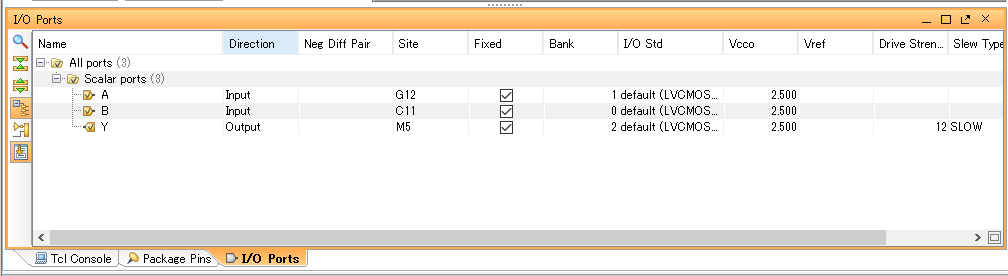
\includegraphics[width=140mm,angle=0]{week2/pics/pinasign.png}
  \centering
   \caption{ANDゲートのピンアサイン} %タイトルをつける
   \label{fig:ANDpinasign} %ラベルをつけ図の参照を可能にする
\end{figure}

\clearpage
%==============================================
\section{実験結果}

\subsection{課題1 3入力多数決回路}
シュミュレーション結果を図\ref{fig:tmrsim}に示す.

\begin{figure}[tbp]
  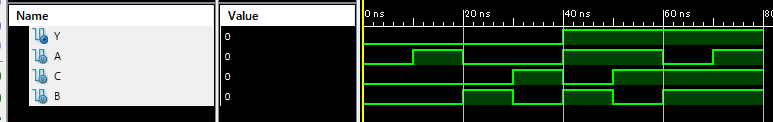
\includegraphics[width=140mm,angle=0]{week2/pics/TMRsim.png}
  \centering
   \caption{3入力多数決回路のシュミュレーション結果} %タイトルをつける
   \label{fig:tmrsim} %ラベルをつけ図の参照を可能にする
\end{figure}


\subsection{課題2 発展課題 10進7セグデコーダの制作}
シュミュレーション結果を図\ref{fig:schbased7segsim}に示す.
テストベンチの結果の中で,赤で引かれた線に注目すると,7セグのデコード結果が見える.
\begin{figure}[tbp]
  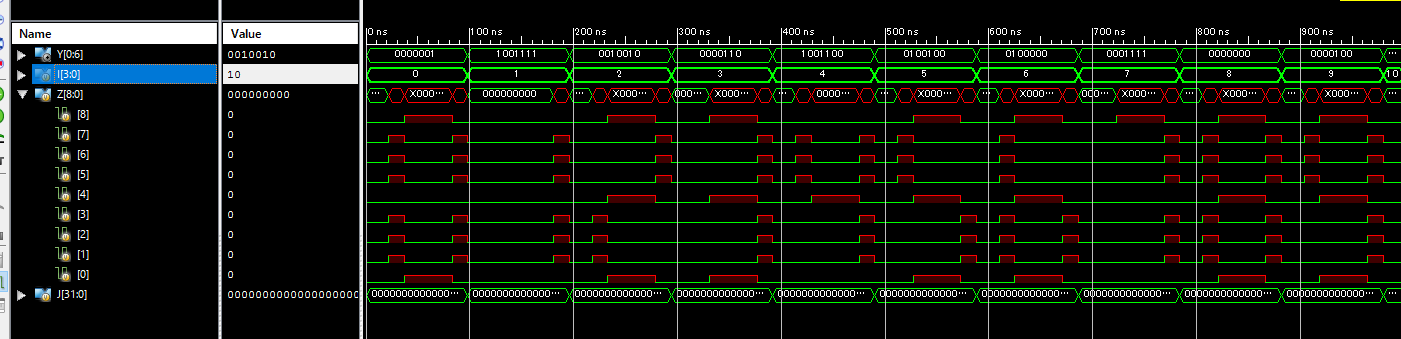
\includegraphics[width=140mm,angle=0]{week2/pics/waveform-7seg.png}
  \centering
   \caption{7セグメントデコーダのモジュールテスト} %タイトルをつける
   \label{fig:schbased7segsim} %ラベルをつけ図の参照を可能にする
\end{figure}


\subsection{課題3 2入力ANDゲートのFPGAボードでの動作確認}
動作確認をしている様子を図\ref{fig:LEDANDex}に示す.
2つのボタンを0個または1個押したときにはLEDは点灯せず,両方のボタンを押したときのみLEDが点灯した.

\begin{figure}[tbp]
  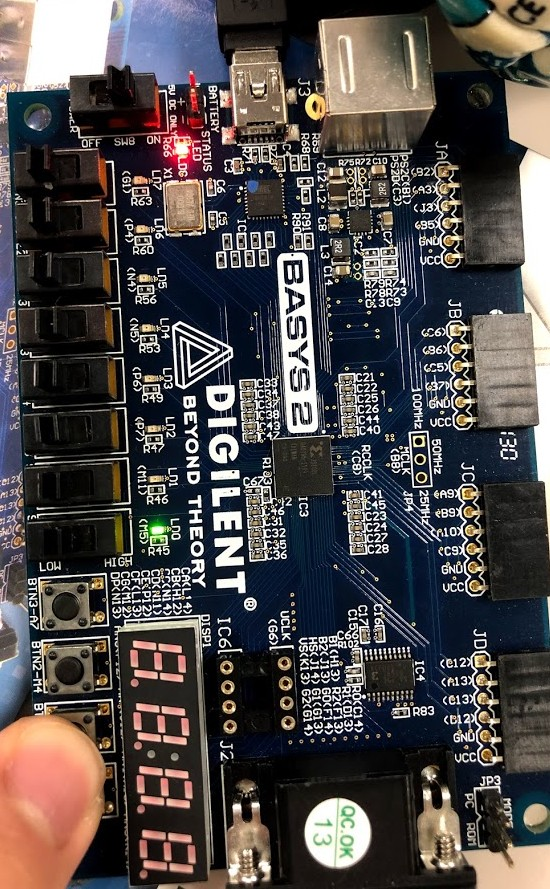
\includegraphics[angle=90,width=140mm]{week2/pics/LEDAND.jpg}
  \centering
   \caption{2入力ANDのLEDへの出力テスト} %タイトルをつける
   \label{fig:LEDANDex} %ラベルをつけ図の参照を可能にする
\end{figure}

\section{考察}
\subsection{課題1 3入力多数決回路}
3入力多数決回路について,予想通りの動作ができていることがわかる.
この回路で,信頼性が求められる計算の正確性が確保できると考えられる.

\subsection{課題2 発展課題 10進7セグデコーダの制作}
7セグメントデコーダも,波形から正しくデコードできている様子がわかる.
0 で光るように設計したため,ANDベースで設計する際に論理素子が少なくて済んだ.
これも,光る部分の設計より,光らない部分を考えたほうが回路が簡略化しやすいことが理由としてある.

\subsection{課題3 2入力ANDゲートのFPGAボードでの動作確認}
2入力 AND 回路について,想定通り両方のボタンを押したときのみLEDが光った.
これは,スイッチが押されたら1,LEDも1のときに光るように設計されているためである.

\section{感想}
コンピュータ上での回路設計に触れることができ,基本的なFPGAの特性をつかむことができた.
特に実際に回路をブレッドボードと論理ゲートで組むことなく,複雑な回路のエミュレートが実機レベルで開発できる点から,
FPGAは有用だと思う.

7セグメントデコーダの制作では,どのセグを光らせるのか,迷う部分があった.
例えば1, 6, 7, 9などは光らせ方が複数あり\footnote{数字''1''は右左の違い,6, 7, 9 はそれぞれA,F,Dセグメントの発光の有無に迷う},
それぞれの数字において,発光パターンが複数考えられたが,
解説に揃えて設計することにした.後の検算のことを考えてのことである.

あと,レポート作成時にTexで表作るのが意外と大変だった.
Excel等で作った表を変換するソフトを用意すべきだと思った.

\clearpage
\section{付録}
\lstinputlisting[caption=TMRのテストベンチ,label=lst:tmrtestbench]{week2/program/TMRtestbench.v}
\lstinputlisting[caption=回路図で設計した7セグデコーダのテストベンチ,label=lst:schbased7segtestbench]{week2/program/schbased7segtestbench.v}
